% in this file I leave the figure captions outside\ caption{} because I want them
% to be formatted in the same way as the general text (double spaced and linenumbered)
\captionsetup[figure]{labelfont={sc},labelformat={default},labelsep=period,name={Figure}}

\begin{figure}[!h]
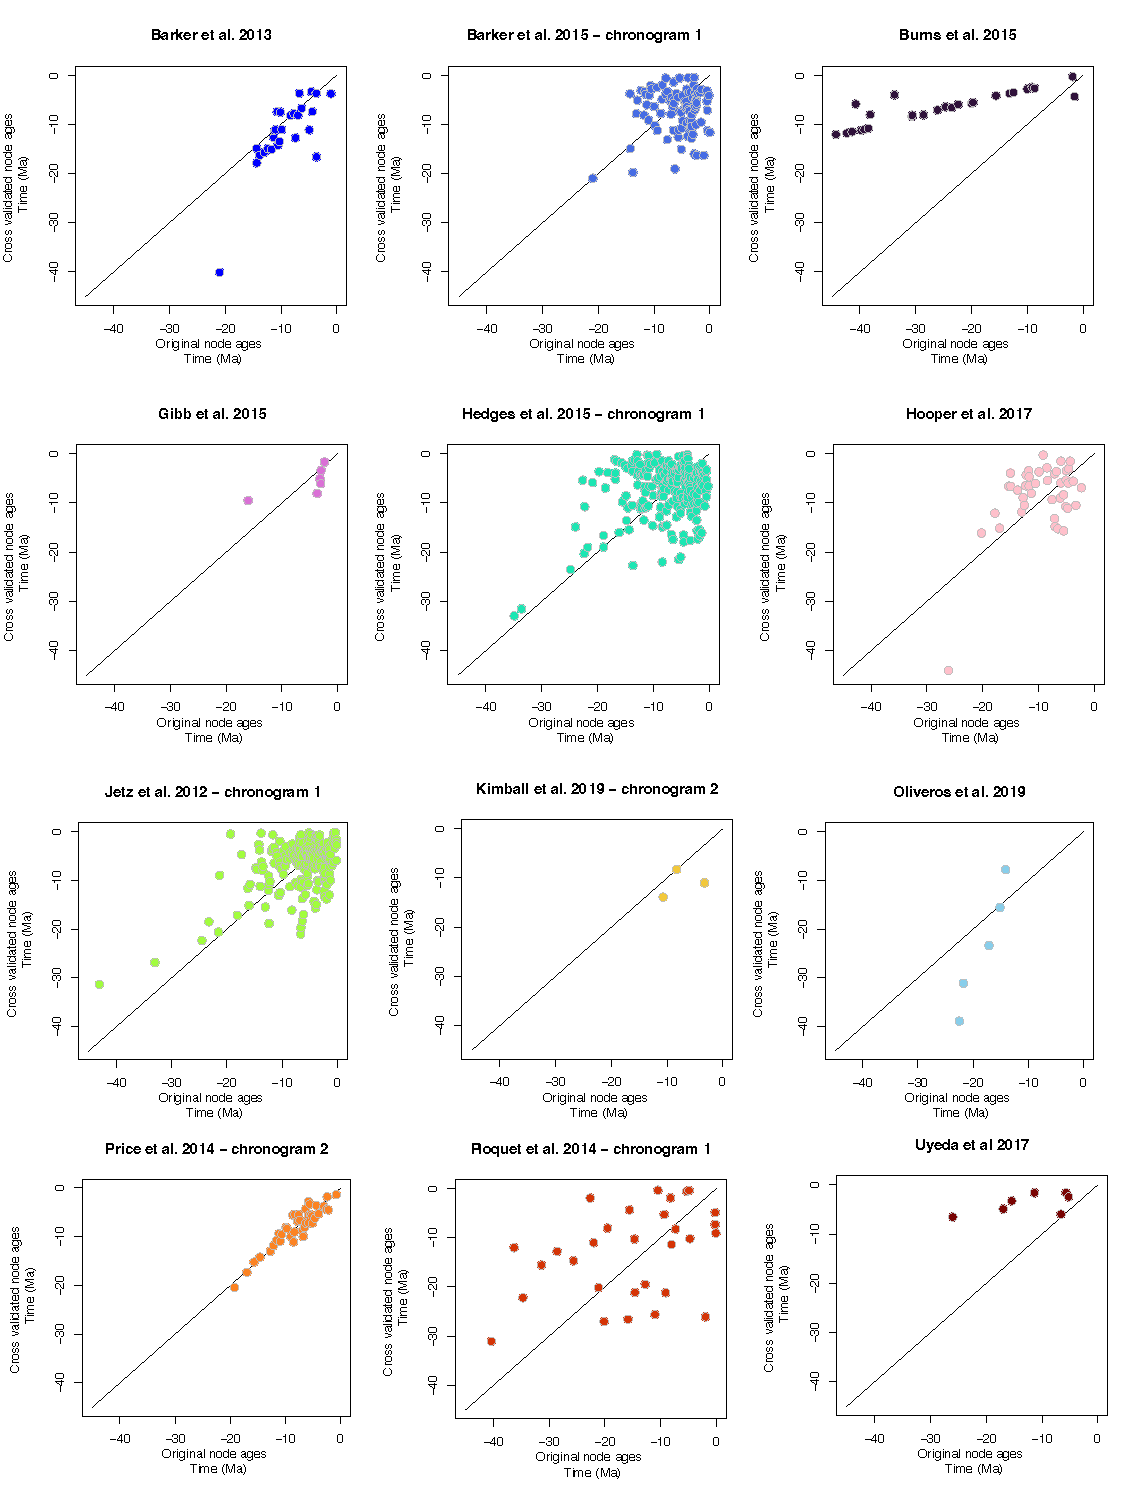
\includegraphics{../figures/figure-cross-validation/fig-cross-validation-xy-plots.pdf}
\caption{Results from cross validation analysis.}
\label{fig:cvXY}
\end{figure}

\begin{figure}[!h]
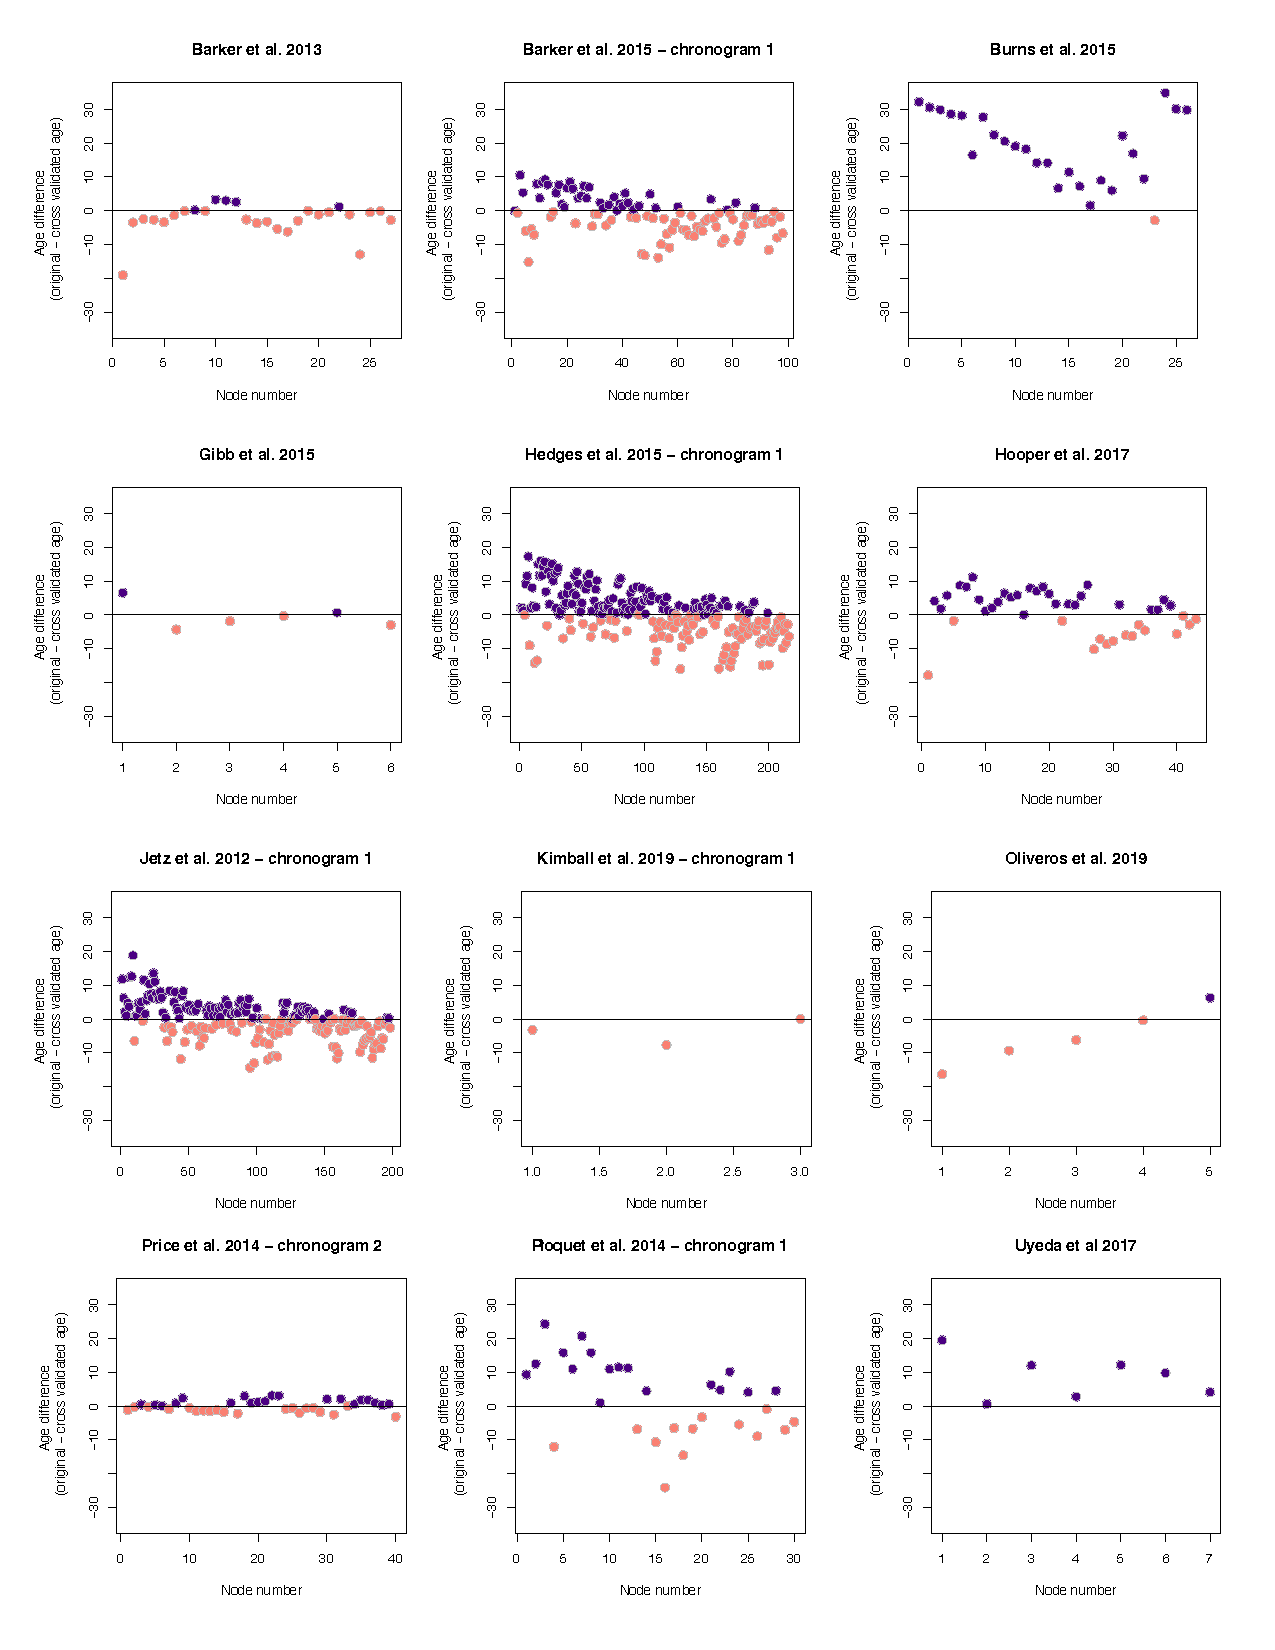
\includegraphics{../figures/figure-cross-validation/fig-cross-validation-xy-plots-diffs.pdf}
\caption{Results from cross validation analysis.}
\label{fig:cvXYdiffs}
\end{figure}

\begin{figure}[!h]
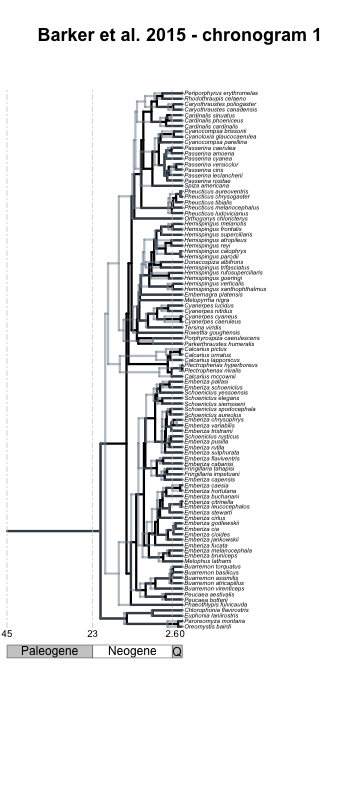
\includegraphics{../figures/figure-cross-validation/cross_validation_2.png}
\caption{Cross validation of second source chronogram. The chronogram shown in black corresponds to the dates published in the original study. The gray chronogram corresponds to the same tree topology dated with BLADJ using node ages from all other source chronograms as secondary calibrations.}
\label{fig:cv2}
\end{figure}

\begin{figure}[!h]
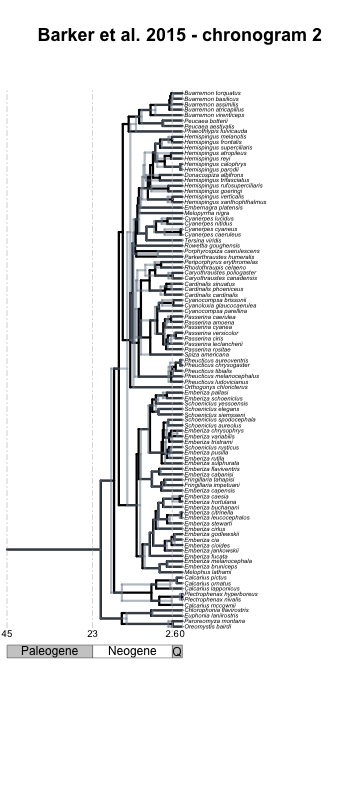
\includegraphics{../figures/figure-cross-validation/cross_validation_3.png}
\caption{Cross validation of third source chronogram. The chronogram shown in black corresponds to the dates published in the original study. The gray chronogram corresponds to the same tree topology dated with BLADJ using node ages from all other source chronograms as secondary calibrations.}
\label{fig:cv3}
\end{figure}

\begin{figure}[!h]
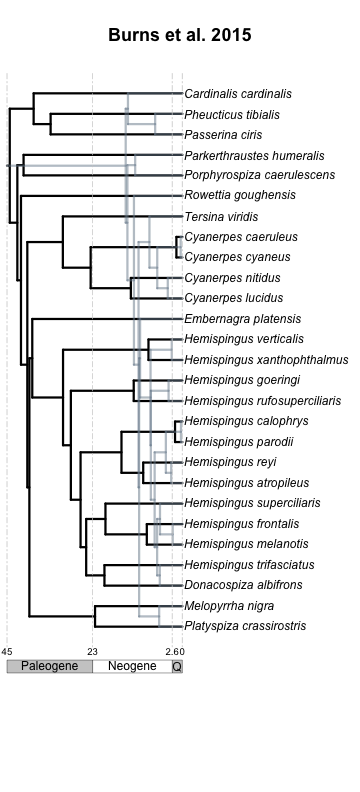
\includegraphics{../figures/figure-cross-validation/cross_validation_4.png}
\caption{Cross validation of fourth source chronogram. The chronogram shown in black corresponds to the dates published in the original study. The gray chronogram corresponds to the same tree topology dated with BLADJ using node ages from all other source chronograms as secondary calibrations.}
\label{fig:cv4}
\end{figure}

\begin{figure}[!h]
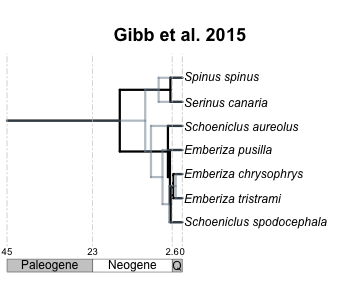
\includegraphics{../figures/figure-cross-validation/cross_validation_6.png}
\caption{Cross validation of sixth source chronogram. The chronogram shown in black corresponds to the dates published in the original study. The gray chronogram corresponds to the same tree topology dated with BLADJ using node ages from all other source chronograms as secondary calibrations.}
\label{fig:cv6}
\end{figure}

\begin{figure}[!h]
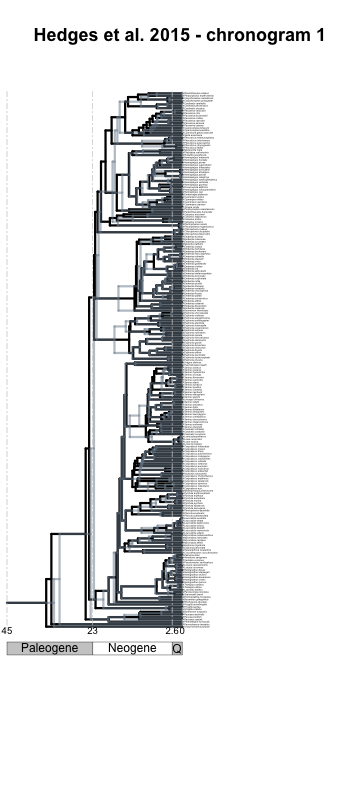
\includegraphics{../figures/figure-cross-validation/cross_validation_7.png}
\caption{Cross validation of seventh source chronogram. The chronogram shown in black corresponds to the dates published in the original study. The gray chronogram corresponds to the same tree topology dated with BLADJ using node ages from all other source chronograms as secondary calibrations.}
\label{fig:cv7}
\end{figure}

\begin{figure}[!h]
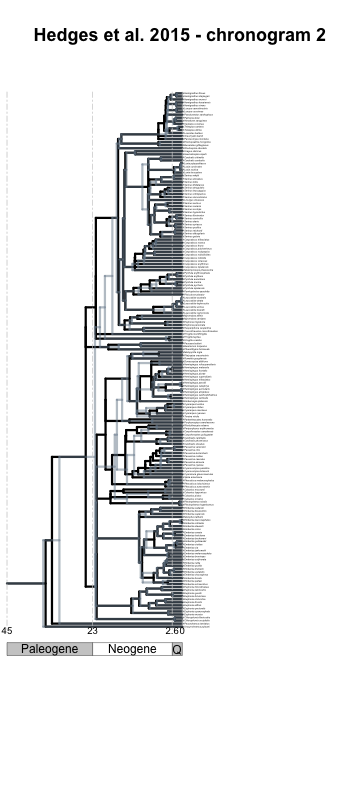
\includegraphics{../figures/figure-cross-validation/cross_validation_8.png}
\caption{Cross validation of eight source chronogram. The chronogram shown in black corresponds to the dates published in the original study. The gray chronogram corresponds to the same tree topology dated with BLADJ using node ages from all other source chronograms as secondary calibrations.}
\label{fig:cv8}
\end{figure}

\begin{figure}[!h]
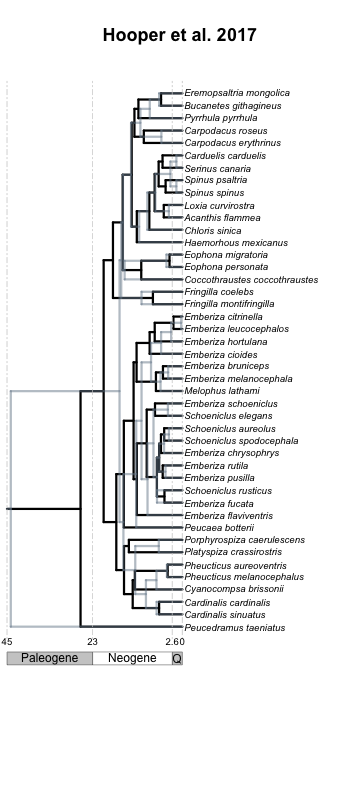
\includegraphics{../figures/figure-cross-validation/cross_validation_9.png}
\caption{Cross validation of ninth source chronogram. The chronogram shown in black corresponds to the dates published in the original study. The gray chronogram corresponds to the same tree topology dated with BLADJ using node ages from all other source chronograms as secondary calibrations.}
\label{fig:cv9}
\end{figure}

\begin{figure}[!h]
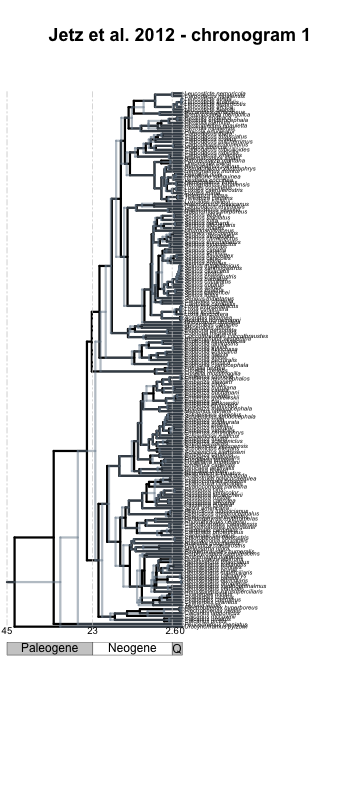
\includegraphics{../figures/figure-cross-validation/cross_validation_10.png}
\caption{Cross validation of tenth source chronogram. The chronogram shown in black corresponds to the dates published in the original study. The gray chronogram corresponds to the same tree topology dated with BLADJ using node ages from all other source chronograms as secondary calibrations.}
\label{fig:cv10}
\end{figure}
